\chapter{Summary and Outlook}
We've measured elliptic flow in p+Au at 200 GeV. This completes a set of measurements with engineered initial collision geometries from RHIC, including p+Au, d+Au, and HeAu as seen in Fig \ref{fig:all_system_hydro_6} . We've measured a significant $v_2$ which is in agreement with Monte Carlo Glauber plus relativistic hydrodynamics.
In the future, work is being done to measure the elliptic flow of the d+Au collision system at 4 energies: 200, 62, 39, 20 GeV. 
\begin{figure}
\begin{center}
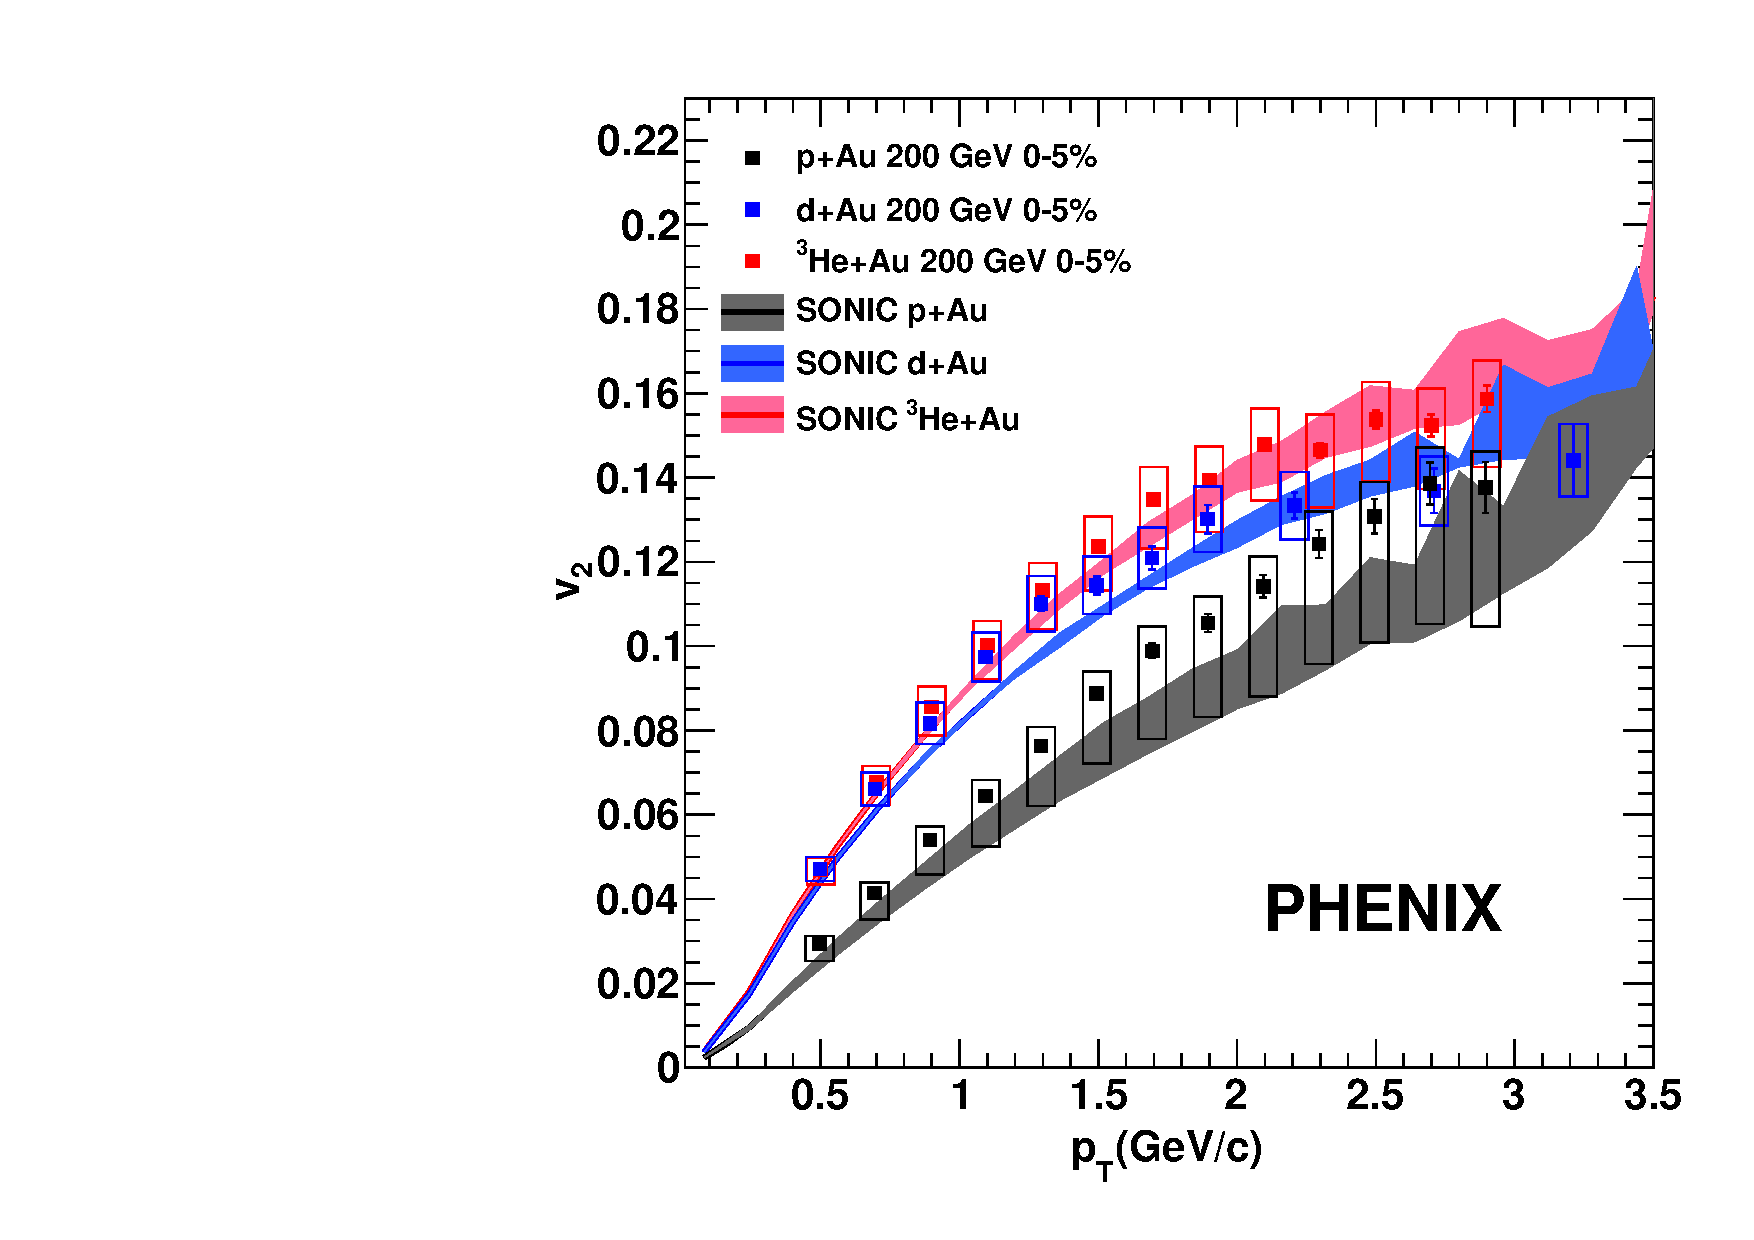
\includegraphics[width=0.5\linewidth]{figs/three_system_comparison_result.pdf}
\caption{$v_2$ of charged hadrons within $|\eta| <$ 0.35 in 0\%--5\% p+Au, d+Au, and HeAu central collisions, compared to hydrodynamic calculations using the \textsc{sonic} model, matched to the same multiplicity as the data. Note that the data points shown include non-flow contributions, whose estimated magnitude is accounted for in the asymmetric systematic uncertainties.}
\label{fig:all_system_hydro_6}
\end{center}
\end{figure}
